%************************************************
\myChapter{Sprzęt}\label{ch:hardware}
%************************************************

Na potrzeby realizacji pracy wymagane było stworzenie sprzętu \pauza urządzenia wejściowego, które będzie pozwalało na śledzenie ruchów palców użytkownika.

Podczas projektowania powstało kilka dodatkowych założeń, które sprzęt powinien spełniać:
\begin{itemize}
 \item łatwość podłączenia \pauza urządzenie powinno być możliwe do ,,zainstalowania'' w kilka chwil, najlepiej bez konieczności korzystania z narzędzi, podłączania zbyt wielu przewodów,
 \item łatwość użytkowania \pauza urządzenie powinno umożliwiać interakcję z komputerem osobom niezapoznanym z pracą, niekoniecznie posiadającym wiedzę techniczną dotyczącą zasady działania,
 \item działanie w możliwie najróżniejszych warunkach \pauza uwzględnienie spodziewanych warunków pracy urządzenia, tak aby nie przeszkadzały one w jego użytkowaniu,
 \item prostota i modułowość \pauza zmniejszenie kosztów produkcji poprzez zastosowanie możliwie prostych, dostępnych i sprawdzonych części połączonych w łatwo wymienialne moduły, co dodatkowo poprawi możliwość zastępowania elementów w wypadku ich uszkodzenia.\\
\end{itemize}

Urządzenie składa się z aluminiowej ramy, złożonej z czterech kątowników, z wywierconymi otworami na diody, fotodiody i elementy mocowania. Rama została zaprojektowana, aby pasowała do posiadanego monitora o przekątnej 24''.

Ramkę w całej okazałości, zamontowaną na wzorcowym monitorze pokazuje rysunek~\ref{fig:frame_full}.

\begin{sidewaysfigure}[!htb]
  \myfloatalign
  \vspace{0.1\textheight}
  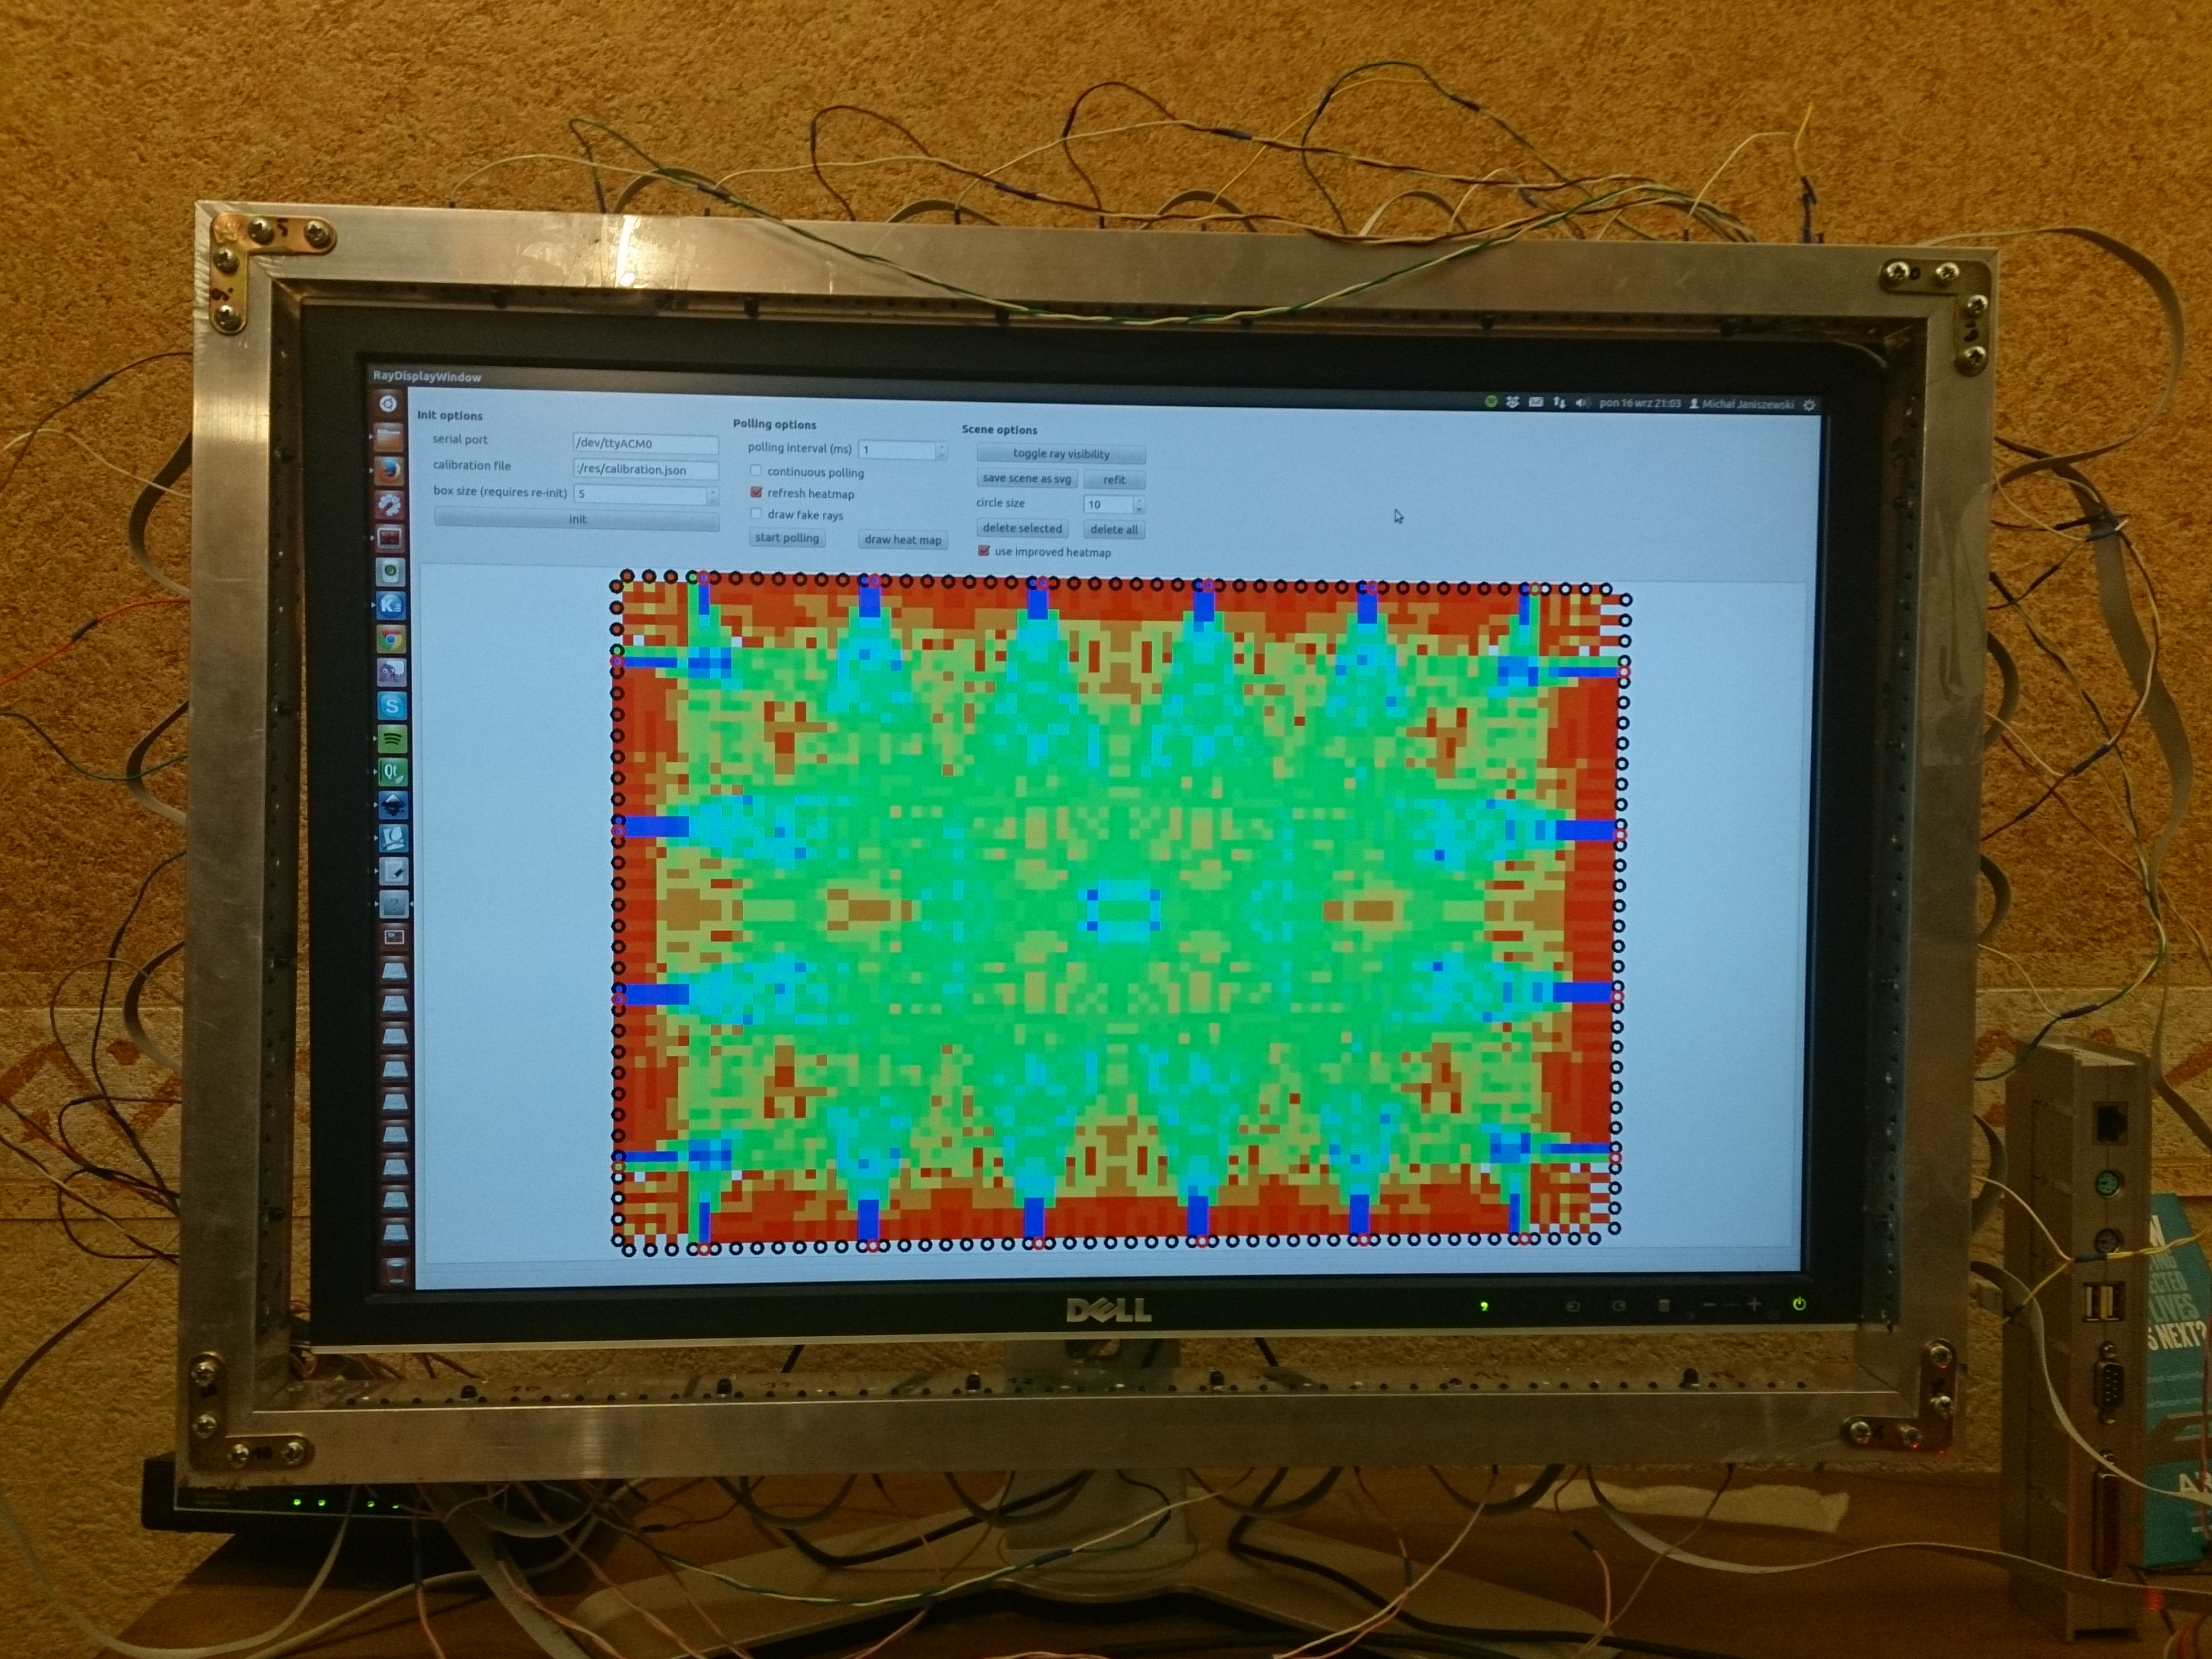
\includegraphics[width=\textwidth]{gfx/frame_full}
  \caption{Ramka zamontowana na docelowym monitorze.}
  \label{fig:frame_full}
\end{sidewaysfigure}

\afterpage{\clearpage}

\section{Moduły nadawczo\ppauza{}odbiorcze.}

Do ramy przymocowanych jest 20 modułów \pauza po 4 na krótsze i po 6~na dłuższe boki. Moduły, ich rozmieszczenie i~sposób montażu prezentuje rysunek~\ref{fig:modules}.

Każdy z jednakowych modułów zawiera komplet elementów do pełnienia funkcji odbiornika oraz nadajnika:
\begin{itemize}
 \item diodę emitującą światło w paśmie podczerwieni (TSAL6400),
 \item 8 fotodiod reagujących na światło wymienionej wyżej diody,
 \item ośmioportowy trzystanowy bufor (74LS541),
 \item zestaw złącz, oporników wymaganych do funkcjonowania powyższych elementów.
\end{itemize}

\begin{figure}[tb]
 \centering
 \makebox[\textwidth][l]{
  \resizebox{.8\largefigure}{!}{
   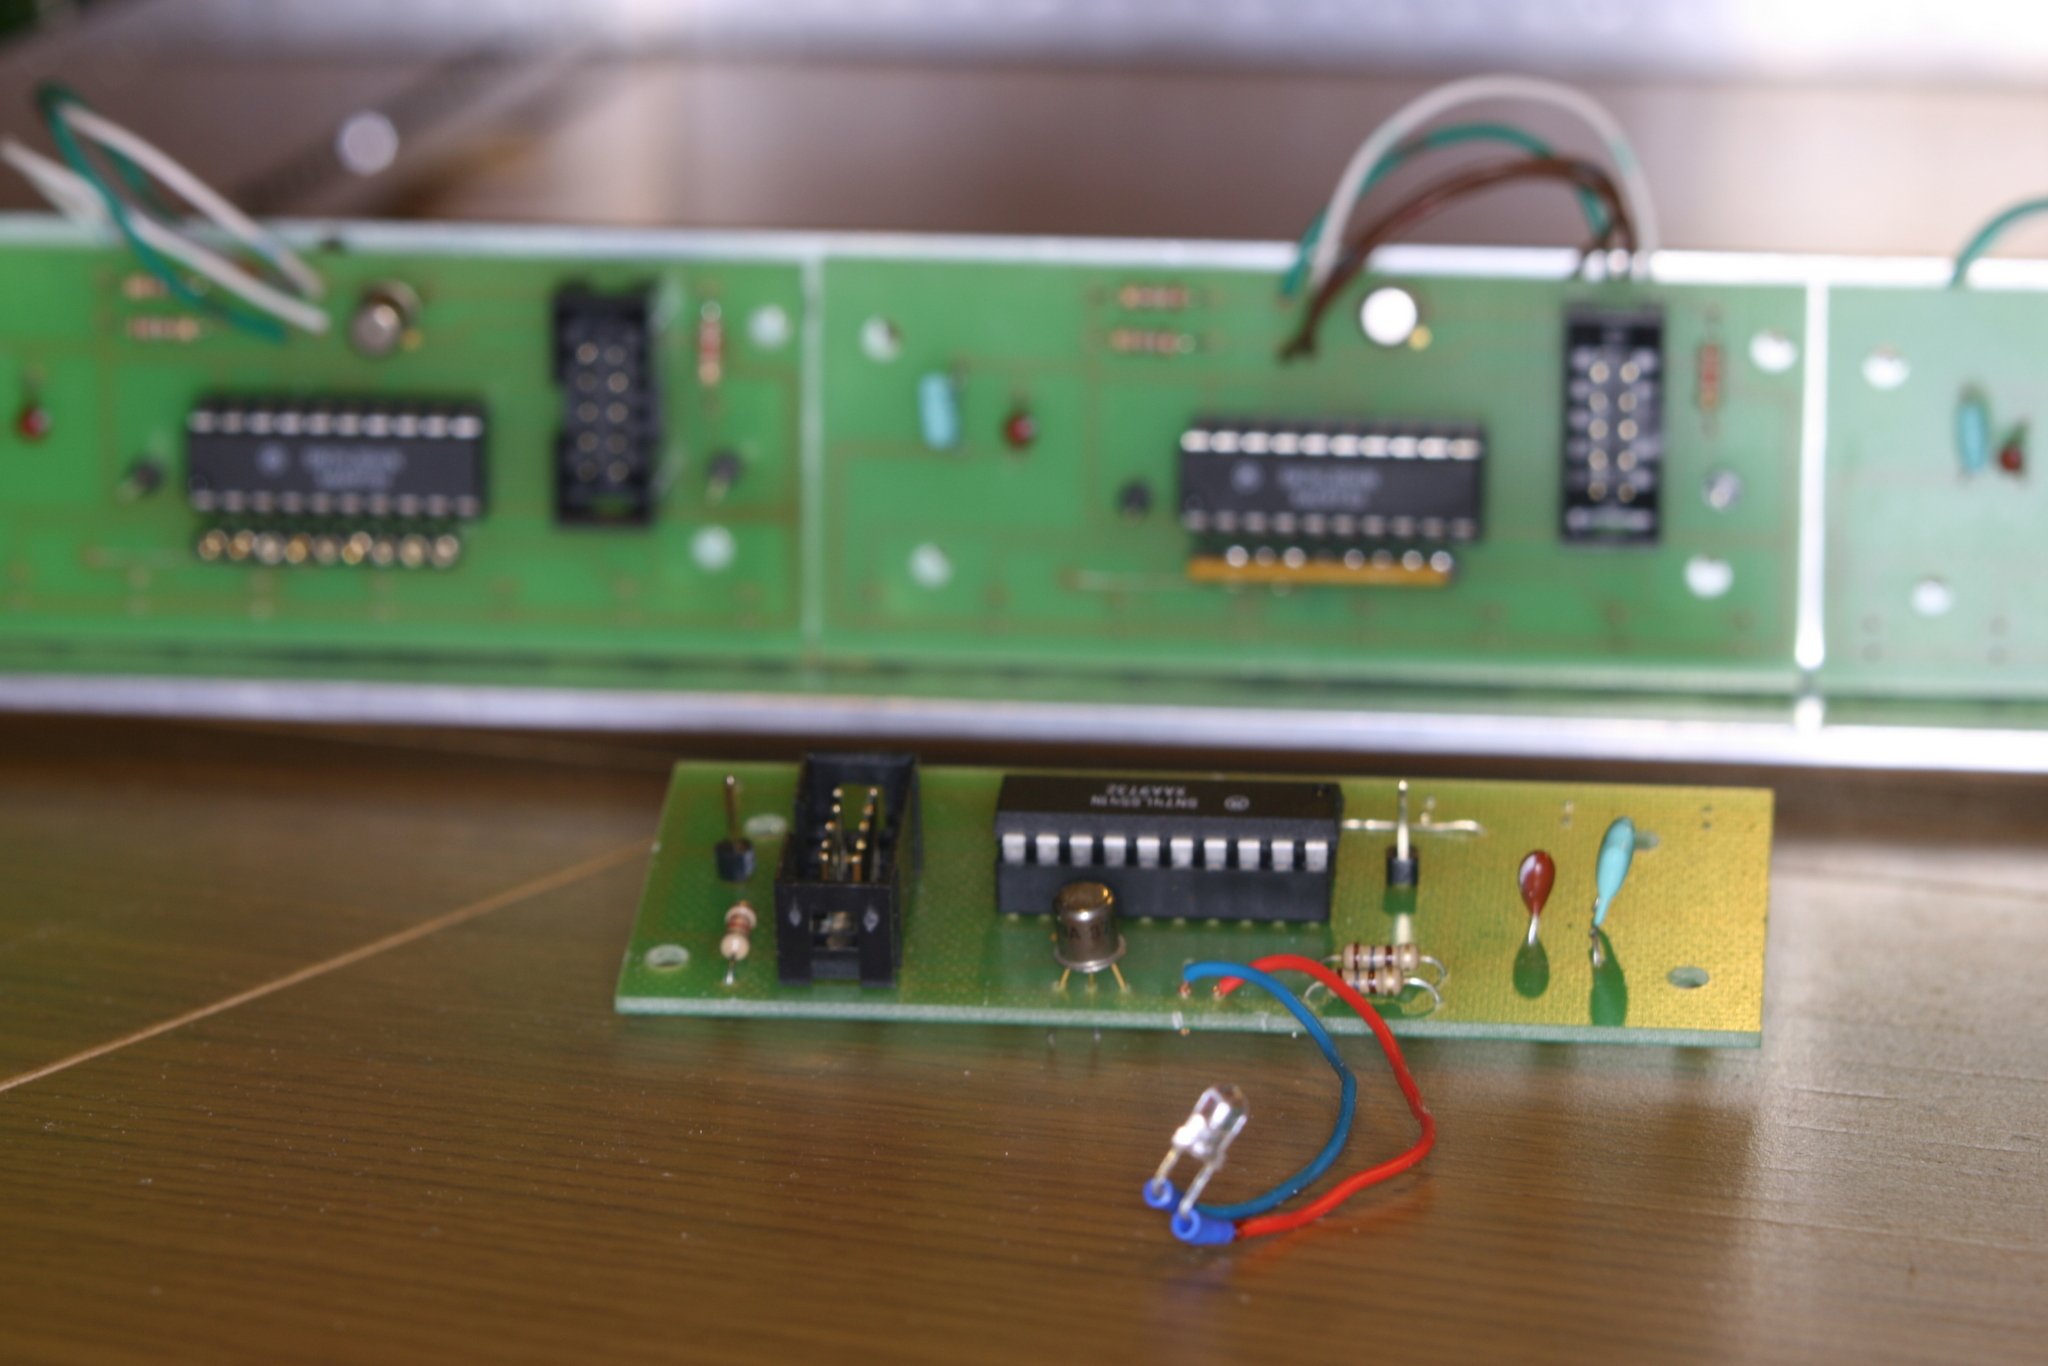
\includegraphics[width=\textwidth]{gfx/modules}
  }
 }
 \caption{Moduły nadawczo\ppauza{}odbiorcze}
 \label{fig:modules}
\end{figure}

Moduły połączone zostały ośmiokanałowym interfejsem równoległym, dodatkowo z dwiema żyłami niosącymi zasilanie oraz osobnymi przewodami z sygnałami chip select (\textsmaller{\textoverline{CS}}) dla bufora oraz diody świecącej (\textsmaller{CS}).\\

Odstęp pomiędzy fotodiodami wynosi 10mm, natomiast między nadajnikami 80mm, co przekłada się na charakterystykę modułów: 8~odbiorników w równych odstępach, 1 nadajnik po środku.
Średnica odbiorników wynosi 3mm, zaś nadajników:
\begin{itemize}
 \item w pierwotnym planie też 3mm, rozmieszczone jeden nad drugim w celu zwiększenia ich widoczności,
 \item w finalnej wersji jeden nadajnik o średnicy 5mm.\\
\end{itemize}

Dodatkowo, nadajniki przesunięte są o 5mm względem rastra wyznaczonego przez odbiorniki, tak aby znajdowały się idealnie pomiędzy fotodiodami.

Moduły zostały zaprojektowane w taki sposób, aby rozmieszczenie fotodiod i nadajników było jednolite, bez względu na granice między modułami. Każdy moduł posiada 4 dodatkowe otwory służace przymocowaniu ich do ramki za pomocą śrub.\\

Otwory na moduły wiercone były w miękkim aluminium wykorzystując wzorzec ze stali, którego wykonanie zostało zlecone zewnętrznej firmie.
Wzorzec ten zawierał otwory nie tylko dla jednego modułu (nadajniki, odbiorniki, elementy mocowania), ale także dwa elementy mocujące poprzedniego modułu, co pozwalało na wygodną synchronizację otworów podczas wiercenia. Wzorzec wiertniczy przedstawiony jest na rysunku \ref{fig:holes_master}. Po prawej stronie widać dwa otwory synchronizacyjne (górny $A_0$ \ppauza montażowy, dolny $B$ \ppauza fotodioda), u góry po środku otwory ($C$) nadajników, otwory $A_1$ do $A_4$ to otwory montażowe, pozostałe to miejsca na fotodiody.\\

\begin{figure}
 \centering
 \makebox[\textwidth][r]{
    \def\svgwidth{\textwidth}
    \includesvg{gfx/holes_master}
  }
 \caption{Wzorzec do wiercenia otworów.}
 \label{fig:holes_master}
\end{figure}

Dwie dwustronne płytki drukowane, przedstawione na rysunku \ref{fig:4515_pcb}, każda z zestawem układów 74HC4514 i 74HC4515, pełnią funkcję demultipleksera portów \pauza układy te to dekodery 4\ppauza{}do\ppauza{}16 z zapadkami (\textsl{latches}), które umożliwiają komunikację z modułami za pomocą znacznie zredukowanej ilości pinów niż byłaby wymagana, gdyby każdy moduł podłączać bezpośrednio.
Zastosowanie takiego rozwiązania jest szybsze niż w przypadku interfejsu szeregowego, np. takiego jak I\textsuperscript{2}C lub SPI, jednak pociąga za sobą konieczność poprowadzenia sygnału \textsmaller{CS} oraz \textsmaller{\textoverline{CS}} do każdego modułu osobno zamiast zintegrowania go w magistrali łączącej wszystkie moduły wygodną do podłączania tasiemką.
Konieczność instalowania w każdym module dekodera takiego interfejsu, ustawiania adresów logicznych modułów, chociaż pozwalałaby na dalsze rozszerzanie ramki o kolejne moduły, zwiększałaby koszty oraz wymagany nakład pracy, rozumianej zarówno przez tworzone oprogramowanie jak i ,,koszt'' działania programu, tj. czasu wymaganego do obsługi wybranego protokołu, zaważyły o ostatecznym wyborze rozwiązania równoległego.

\begin{figure}
  \centering
  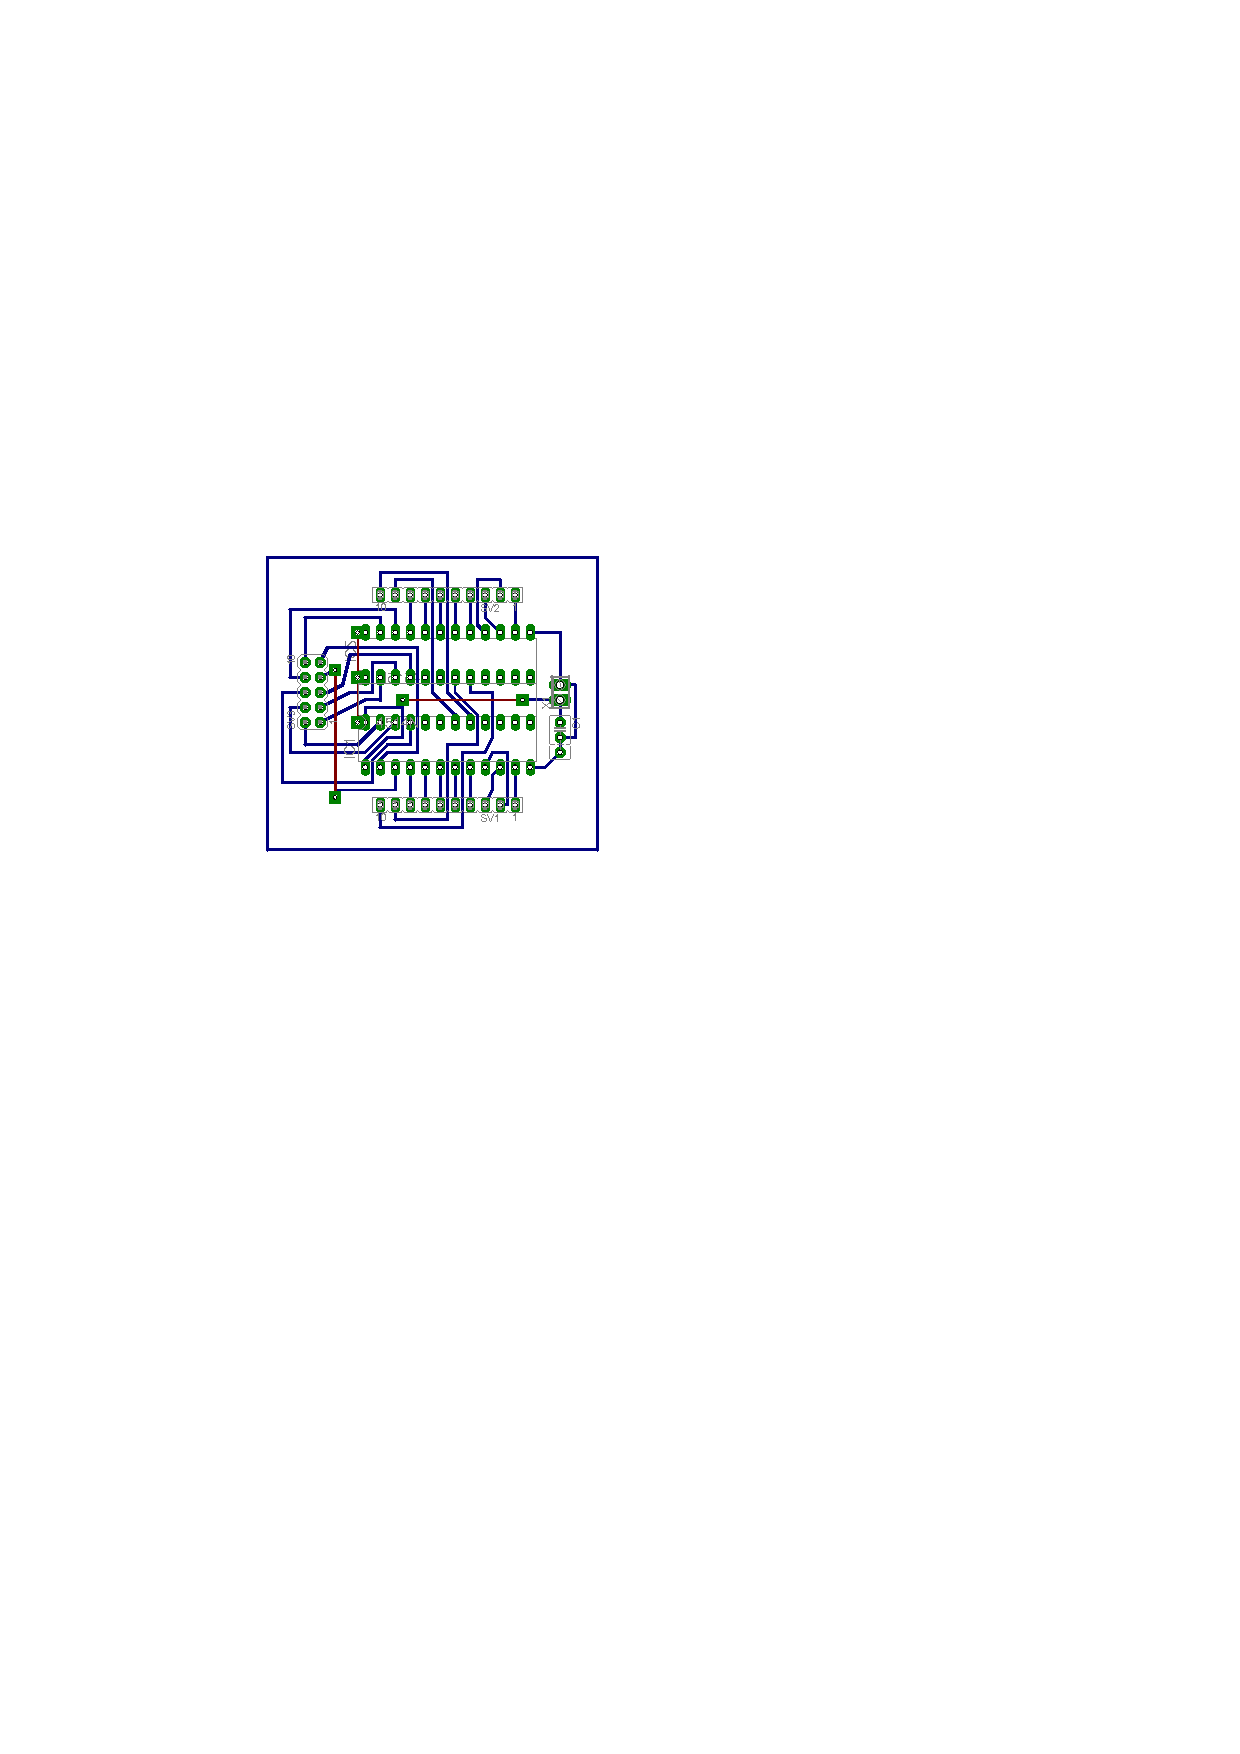
\includegraphics{gfx/4515_drvpcb}
  \caption{Schemat płytki drukowanej z układami 4515/4514.}
  \label{fig:4515_pcb}
\end{figure}

Wszystkie płytki PCB\graffito{PCB, printed circuit board \ppauza płytka z~układem drukowanym.}, z wyjątkiem modułu mikrokontrolera, zostały zaprojektowane i wykonane wyłącznie w celu realizacji pracy.

Stworzony sprzęt przeszedł kilka zmian: zarówno mikroprocesor jak i elementy konstrukcji były kilkukrotnie wymieniane.\\

\section{Rewizja pierwsza}

W pierwszej wersji do kontroli modułów i interfejsowania z komputerem wykorzystany został mikrokontroler z 16-bitowej rodziny MSP430: MSP430FG4618 znajdujący się w płytce Experimenter's Board.
Pod kątem tego urządzenia projektowane były wszystkie interfejsy, uwzględniając przede wszystkim ilość dostępnych pinów oraz charakterystykę prądową.
Płytkę tę prezentuje rysunek~\ref{fig:msp430_exp}.

\begin{figure}
%  \centering
%  \makebox[\textwidth][r]{
%   \resizebox{.9\largefigure}{!}{
%   }
%  }
 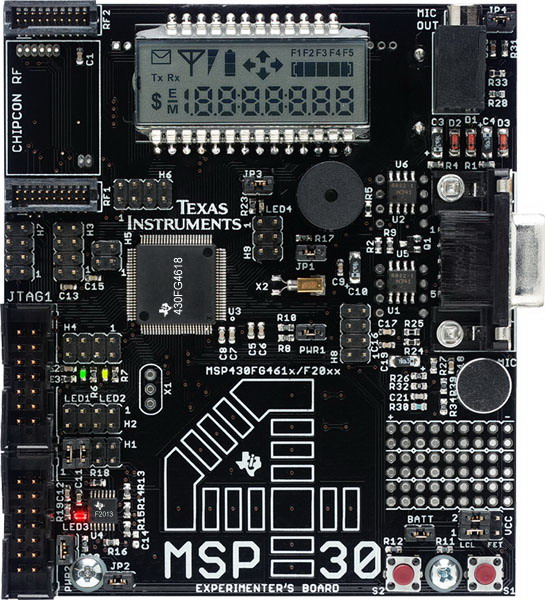
\includegraphics[width=\textwidth]{gfx/exp43000}
 \caption{Płytka MSP430 experimenter's board.}
 \label{fig:msp430_exp}
\end{figure}

\begin{figure}
 \centering
 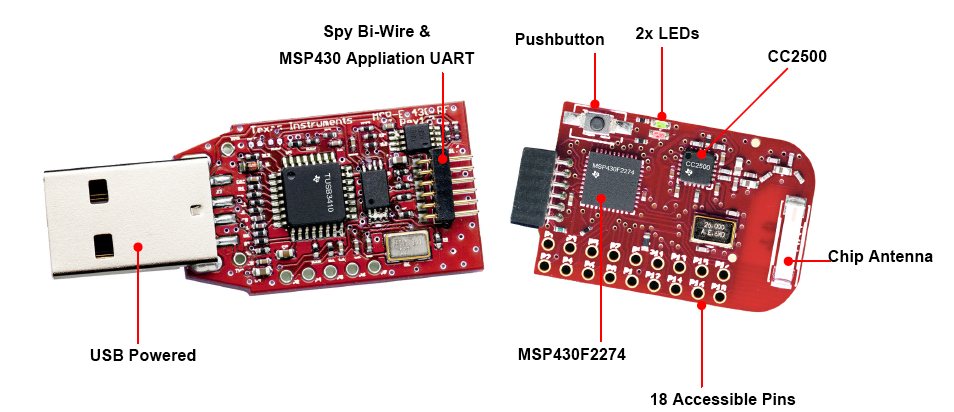
\includegraphics[width=\textwidth]{gfx/ez430-rf2500}
 \caption{Płytka MSP430 eZ430-rf2500}
 \label{fig:msp430_ez430}
\end{figure}

Duże problemy okazał się powodować moduł komunikacji szeregowej UART, który operował w standardzie RS232/TTL\graffito{TTL, transistor\ppauza{}to\ppauza{}transistor logic, poziomy napięć i~prądów przystosowane do niedługich połączeń pomiędzy układami}.
Po podłączeniu adaptera USB\ppauza{}RS232 opartego o renomowany układ FTDI FT2232C okazało się w testach, że podczas dużego obciążenia hosta, pojedyncze bity ramki RS232 mogą się ,,zgubić'', tj. jedynki sporadycznie zastępowane były zerami.
Ze względu na spodziewany charakter wykorzystywania pracy, np. podczas gier, oczekiwane było poprawne działanie także w warunkach wysokiego obciążenia, co dyskwalifikowało takie rozwiązanie.\\

\section{Rewizja druga}

Z powodu dostępności płytki eZ430-RF2500 chciałem wykorzystać zawarty na niej układ MSP430F2274, który mógłby zapewnić spodziewaną stabilność transmisji danych.
Płytka ta podłączana była do komputera bezpośrednio do portu USB, co pozwalało przypuszczać, że wykorzystując inny, znacznie nowszy, podsystem komputera, będzie on działał poprawnie.
Pomimo przeprojektowania płytki interfejsu ramka $\leftrightarrow$ mikrokontroler, która ograniczała liczbę wymaganych połączeń z 24 do 20 \pauza możliwie najniższej praktycznie osiągalnej ilości niewymagającej połączeń szeregowych, układ nie miał nawet takiej ilości złącz GPIO\graffito{GPIO, general-purpose input/output, \pauza interfejs wejścia/wyjścia}.
Ponadto prędkość transmisji była sztucznie ograniczona do wartości 9600BPS, która nie zapewnia wymaganej przepustowości.

Płytkę widać na rysunku~\ref{fig:msp430_ez430}.\\

\section{Rewizja trzecia}

Ze względu na problemy z komunikacją, zdecydowałem się wykorzystać do pracy nowy układ z rdzeniem ARM Cortex\ppauza{}M4F, Texas Instruments LM4F120H5QR na płytce Stellaris Launchpad. Jest to 32-bitowy procesor, dostępny dopiero od listopada 2012, tj. kilka miesięcy po rozpoczęciu pisania pracy.
Układ ten posiada zintegrowany kontroler urządzenia USB pozwalający na uzyskanie niezawodności komunikacji na zadowalającym poziomie.
Moduł pokazany jest na rysunku~\ref{fig:stellaris_launchpad}.

\begin{figure}
 \centering
 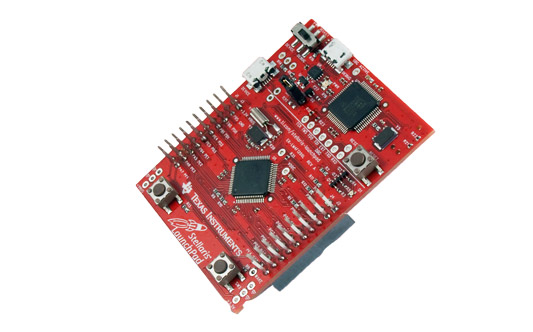
\includegraphics[width=\textwidth]{gfx/stellaris_launchpad}
 \caption[Płytka Stellaris Launchpad]{Płytka Stellaris Launchpad z układem TI LM4F120H5QR}
 \label{fig:stellaris_launchpad}
\end{figure}

Dopiero uzyskanie tego układu pozwoliło na dalszy postęp prac. Problemy związane z brakiem odpowiedniego sprzętu i funduszy na zakup mocniejszych układów były główną przyczyną rozciągnięcia się pracy w czasie.\\

\section{Rewizja czwarta}

W tej wersji, zmieniona została konstrukcja samej ramki i modułów. Pierwotny projekt zakładał, że diody emitujące światło znajdować będą się w innej płaszczyżnie niż elemnty odbiorcze w celu uniknięcia problemu odbić. Moc wykorzystanych wtedy diod okazała się niewystarczająca do poprawnego oświetlenia odbiorników, przesunięte zostały więc one do płaszczyzny odbiorników.

Z powodu nadal niedostatecznej ilości mocy diod, wymienione zostały na modele 5\texttimes\  mocniejsze, używające 120mA: TSAL6400. Dodane także zostały (do niektórych modułów) diody świecące w paśmie światła widzialnego, element nieprzewidziany w pierwotnym projekcie, co pozwoliło na prostsze debugowanie działania urządzenia.\\

\section{Interfejs ramka $\leftrightarrow$ mikrokontroler}

Interfejs zapewniający komunikację między mikrokontrolerem, a~ram\-ką przeszedł tylko jedną wymianę, mającą na celu przede wszystkim wspomniane już ograniczenie ilości wymaganych pinów do obsługi.

Pierwsza wersja oparta była na układach 74LS139 (podwójny selektor 1\ppauza{}z\ppauza{}4) oraz 74LS14 (inwerter), posiadała także zestaw diod LED i oporników pomocnych w debugowaniu. Działanie tego urządzenia było bardzo proste, polegało na wyborze odpowiedniego modułu (nadawczego i odbiorczego) poprzez ustawienie sygnałów \textsmaller{CS} oraz \textsmaller{\textoverline{CS}} po wybraniu danego układu oraz ,,wysłania'' do niego adresu jednej z czterech linii wyjściowych. Sygnał \textsmaller{\textoverline{CS}} uzyskany został przez zastosowanie inwertera 74LS14.

Płytkę tę przedstawia rysunek~\ref{fig:first_interface}.
Na tym rysunku płytka jest rozłączona.\\

Druga, a zarazem finalna wersja tego sprzętu wykorzystuje w tym celu dwie płytki PCB, każda zawierająca po jednym układzie 74HC4514 oraz 74HC4515. Układy te to selektory 1\ppauza{}z\ppauza{}16, które różnią się tylko i wyłącznie wbudowanym inwerterem: 74HC4514 posiada wolną jedynkę, tzn. na wybranym wyjściu ustawiony zostanie stan wysoki, pozostałe linie mają stan niski; układ 74HC4515 posiada wolne zero \pauza na każdej linii znajduje się inwerter.

Ta płytka, podobnie jak jej poprzednia wersja, zawiera zestaw diod LED umożliwiających debugowanie.

Rysunek~\ref{fig:second_interface} przedstawia drugą wersję płytki interfejsowej. Płytka ta na zdjęciu jest podłączona.\\

\begin{figure}
 \centering
 \makebox[\textwidth][l]{
  \resizebox{.8\largefigure}{!}{
   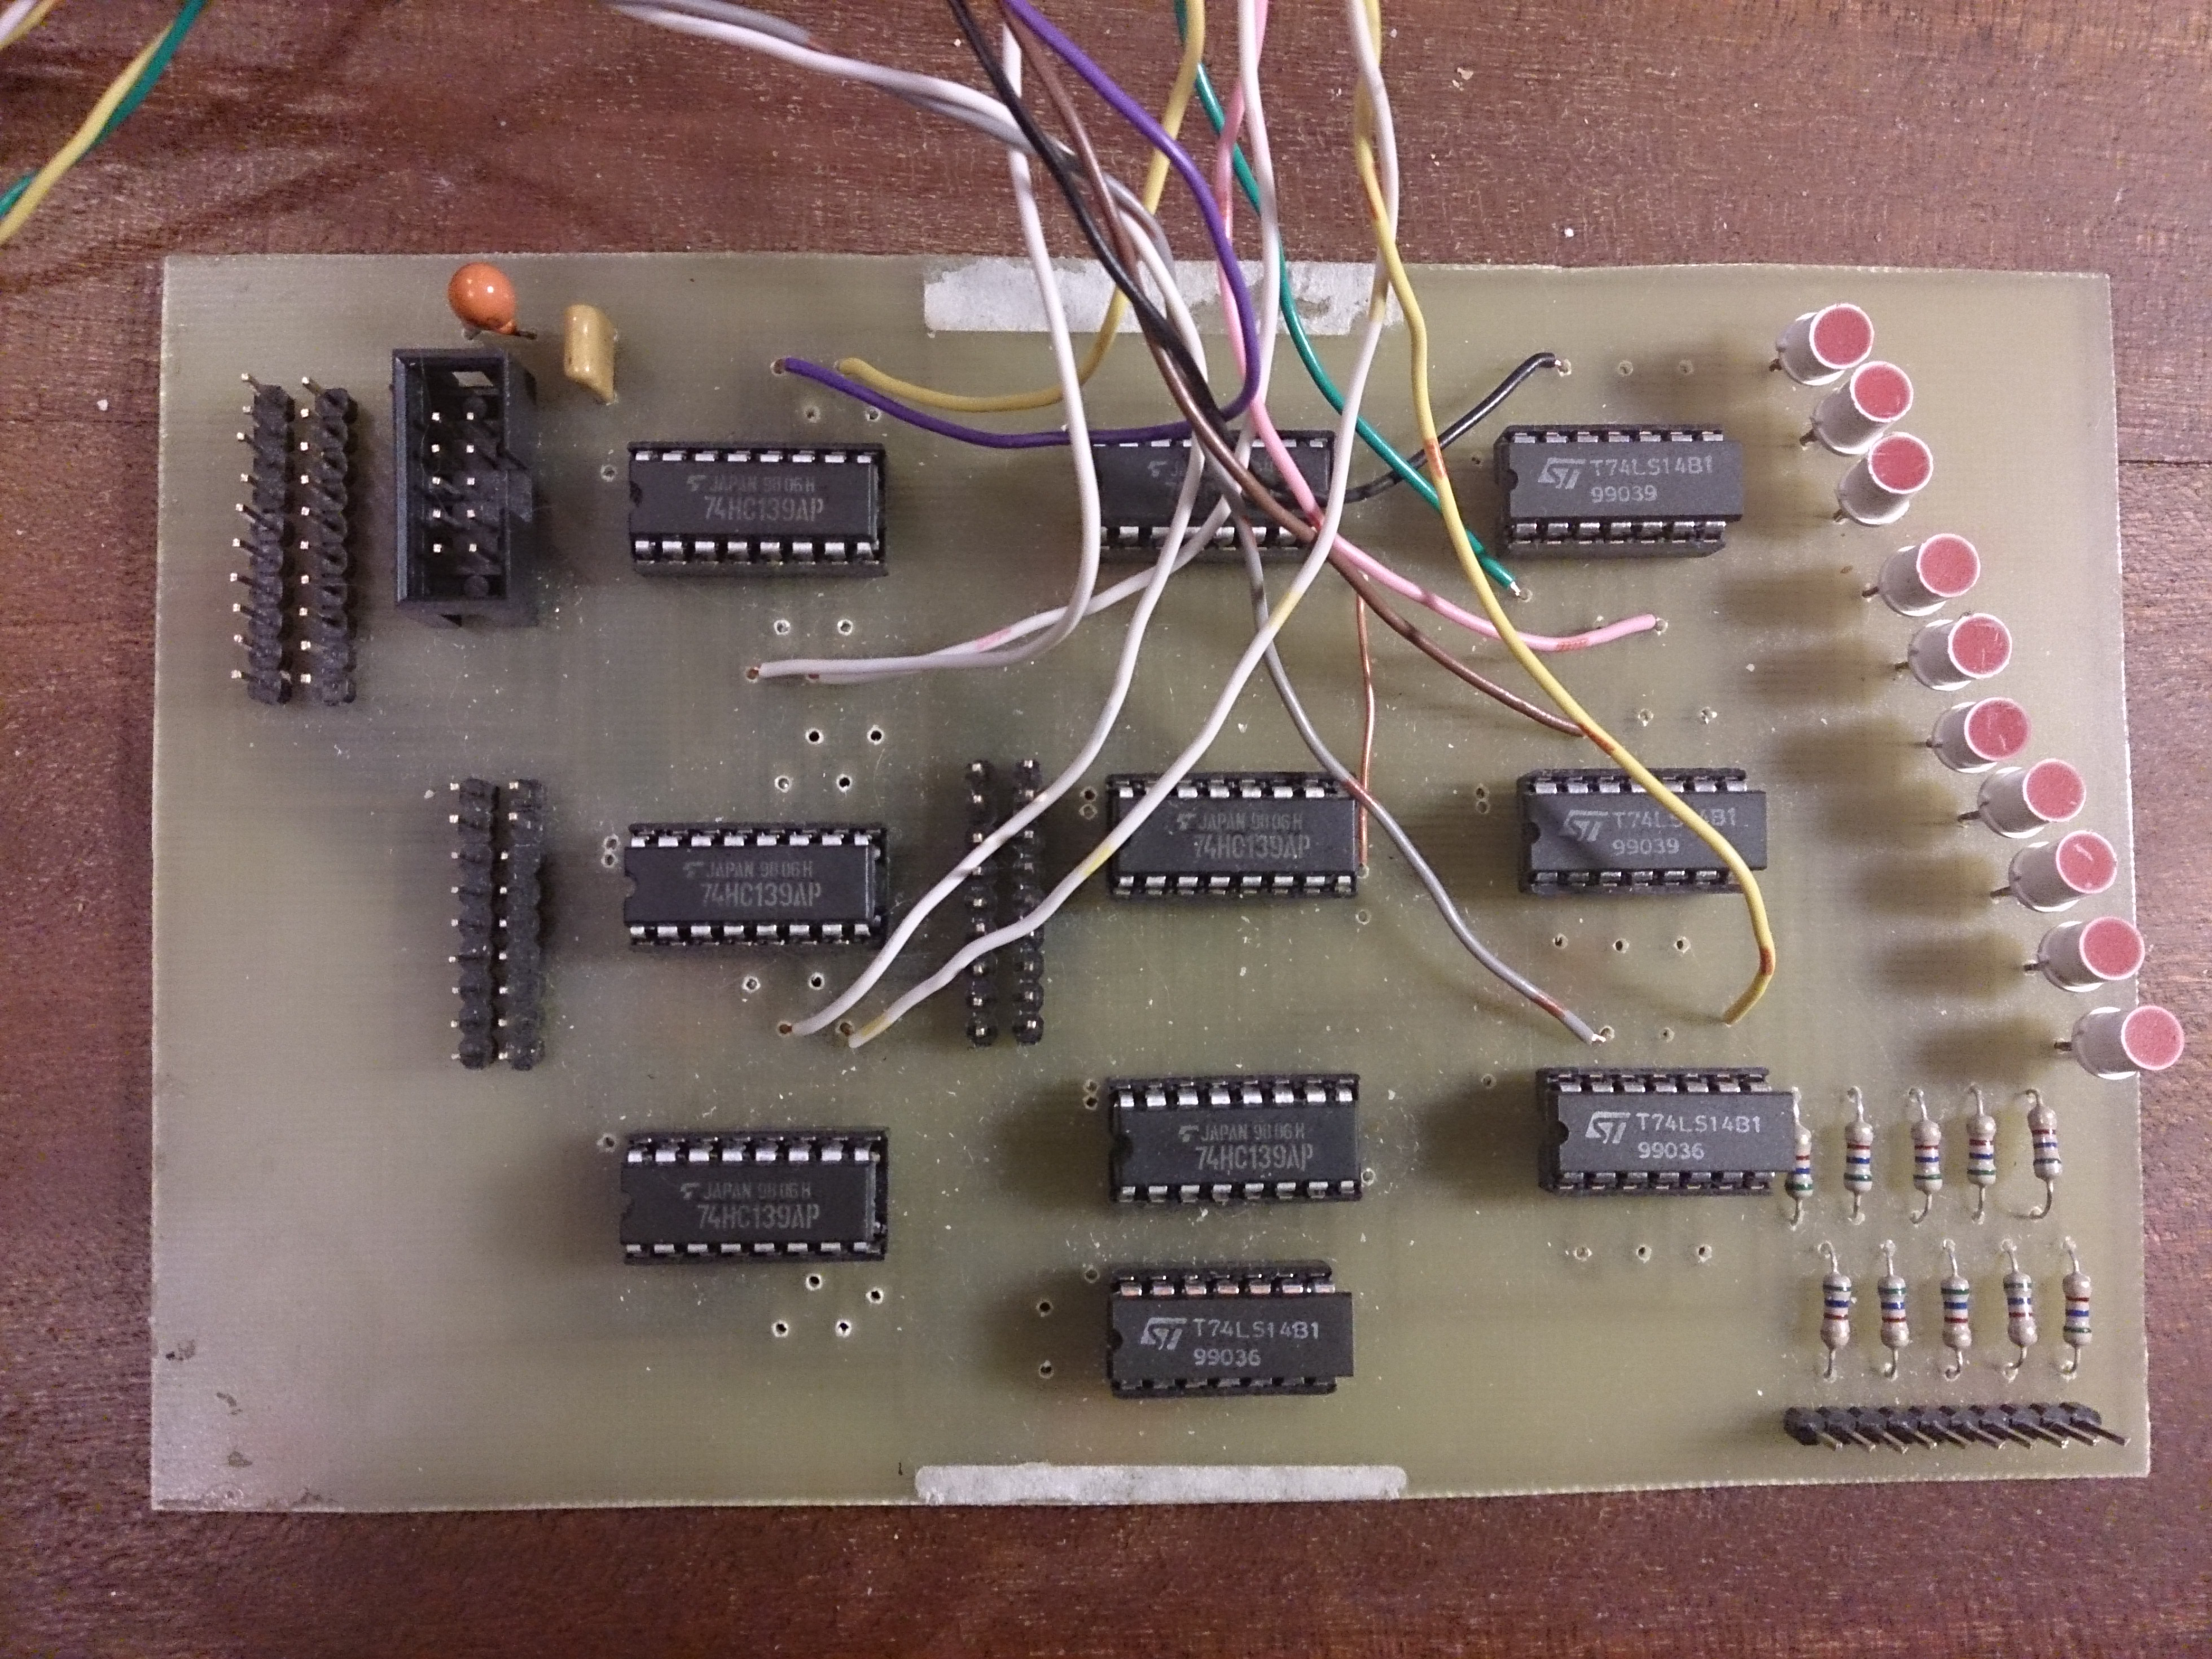
\includegraphics[width=\textwidth]{gfx/first_interface}
  }
 }
 \caption[Pierwsza wersja płytki interfejsowej]{Pierwsza wersja płytki interfejsowej (rozłączona).}
 \label{fig:first_interface}
\end{figure}

\begin{figure}
 \centering
 \makebox[\textwidth][l]{
  \resizebox{.8\largefigure}{!}{
   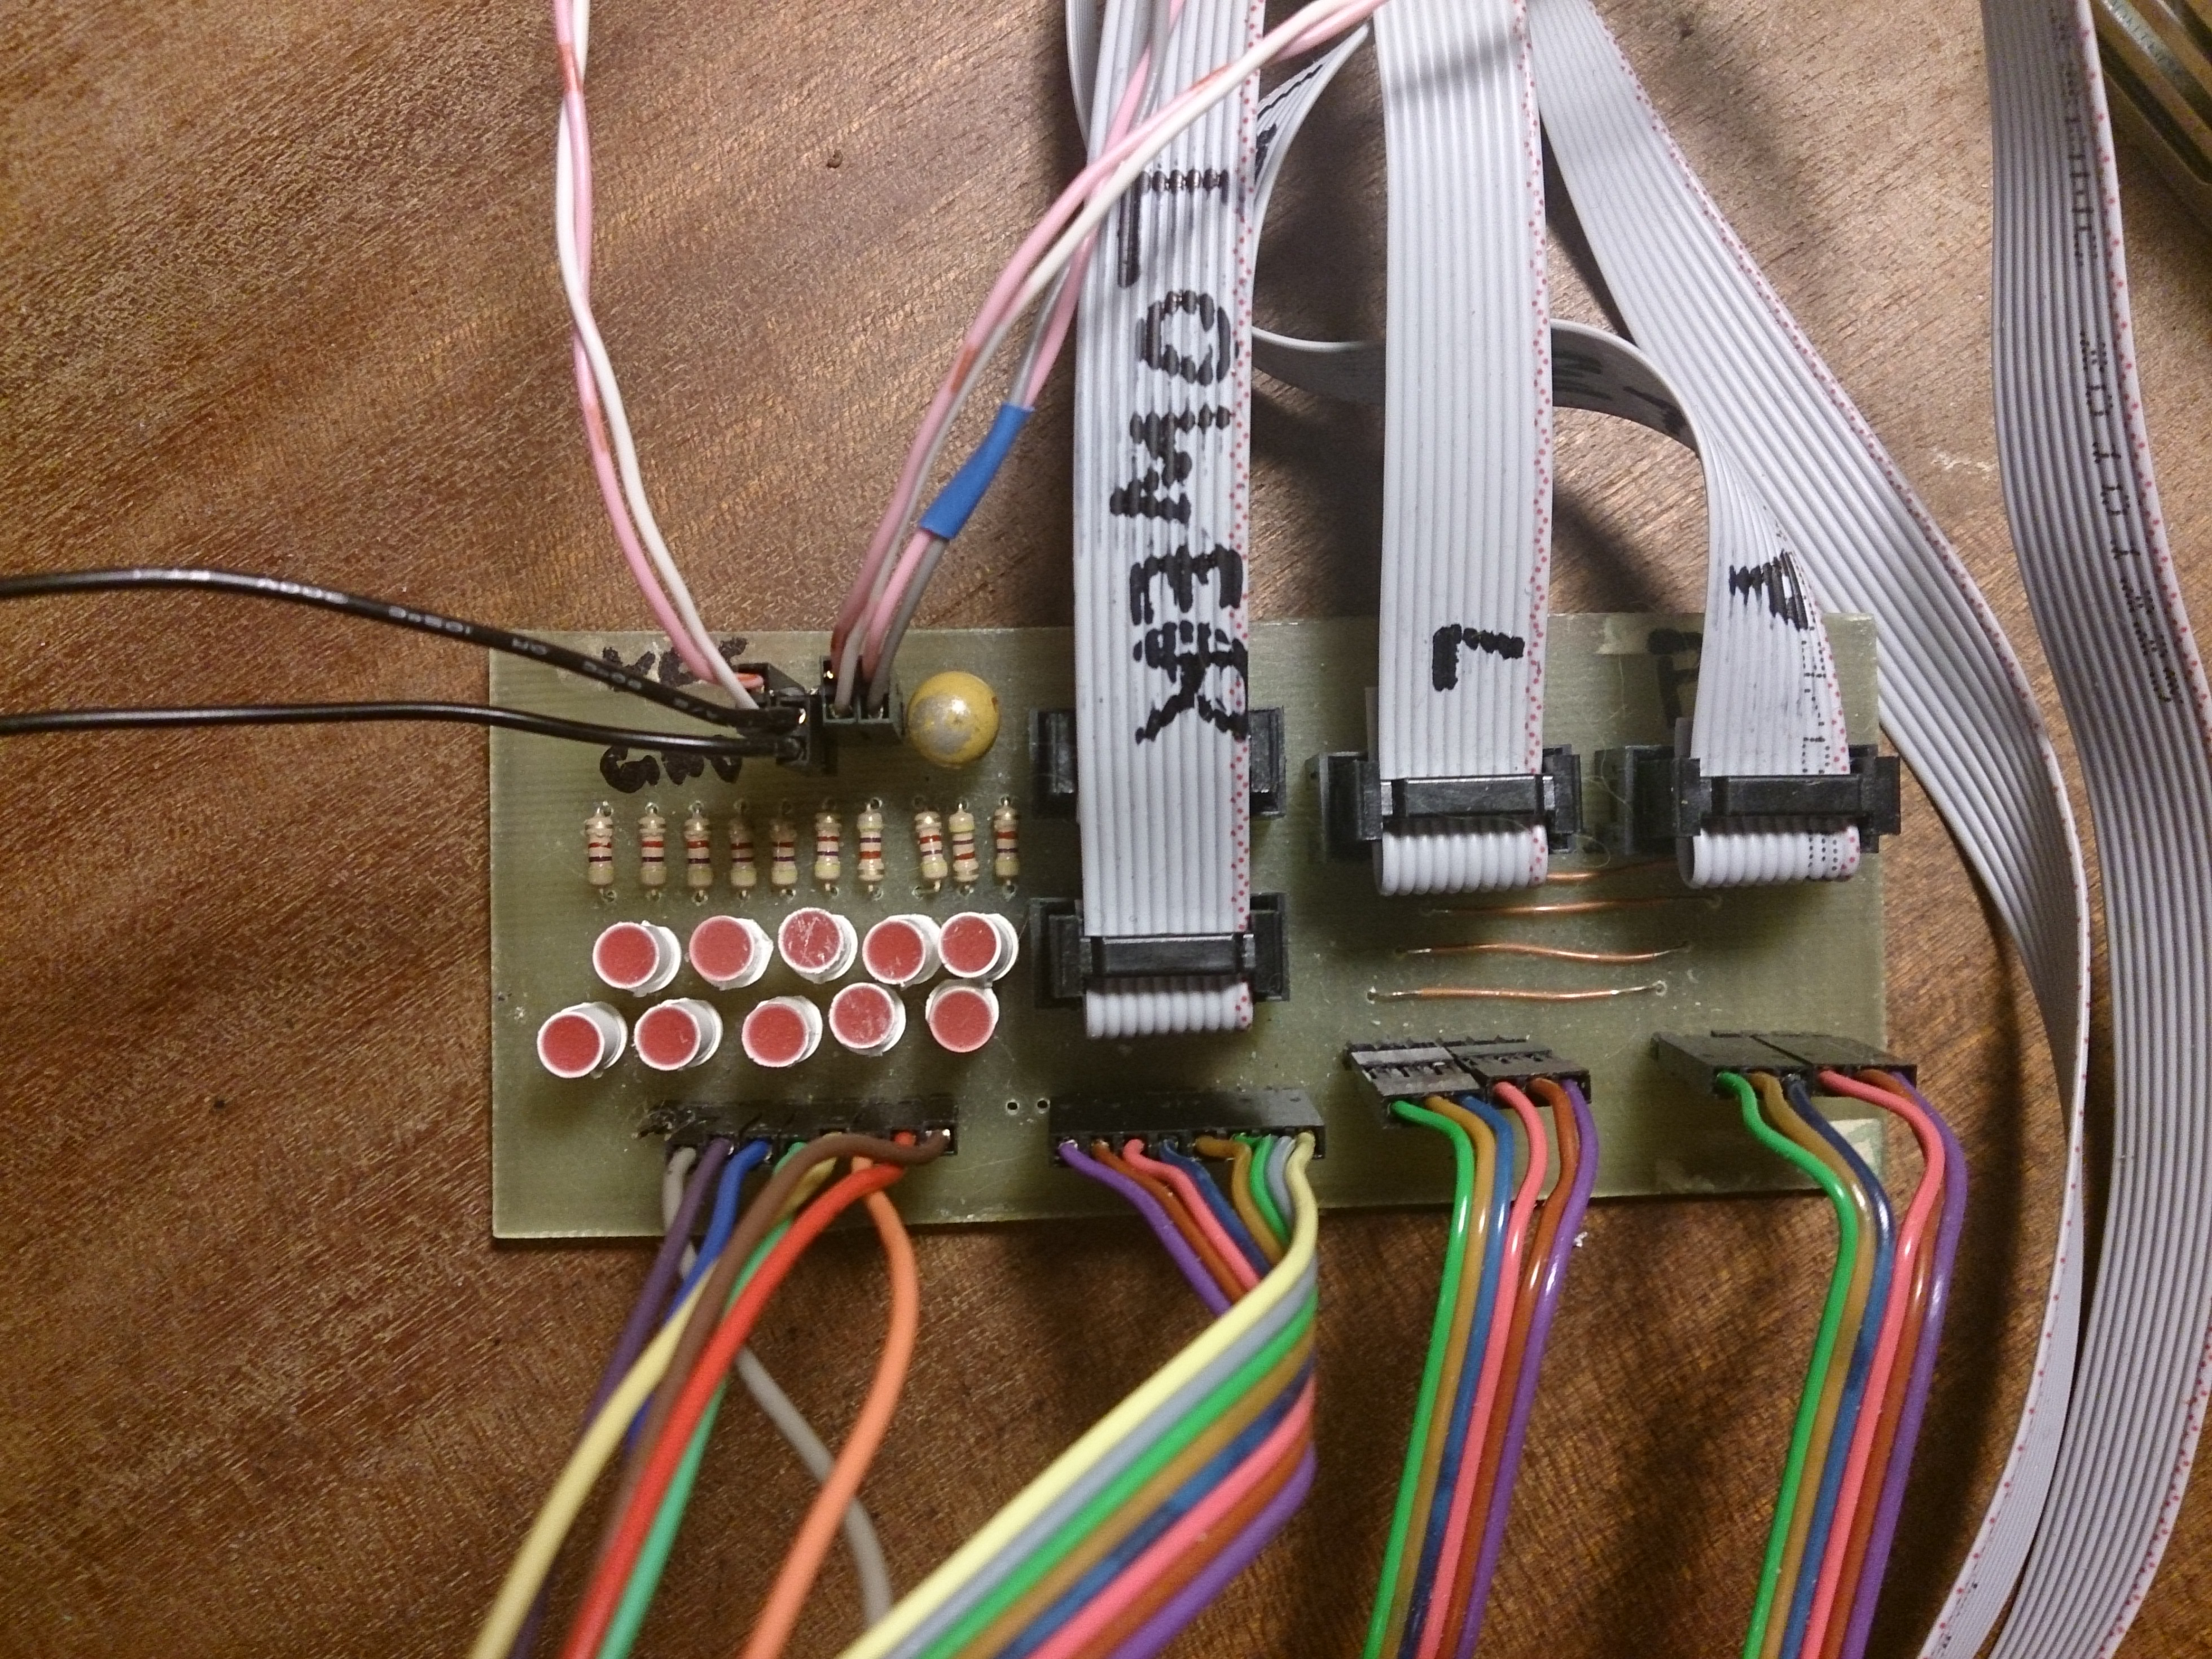
\includegraphics[width=\textwidth]{gfx/second_interface}
  }
 }
 \caption[Druga wersja płytki interfejsowej]{Druga wersja płytki interfejsowej (podłączona).}
 \label{fig:second_interface}
\end{figure}

Zastosowanie dwóch selektorów 16-liniowych wymaga sześciu linii: 4 linie adresowe oraz po jednej linii \textsmaller{\textoverline{I}} (\textsmaller{\textoverline{Inhibit}}) dla każdego układu.
Chociaż 20 użytych modułów można zaadresować za pomocą 5\ppauza{}bitowej przestrzeni adresowej zdolnej do obsługi maksymalnie 32 odbiorników, to należy zwrócić uwagę, że dekodery 5\ppauza{}do\ppauza{}32 nie istnieją.
Ich konstrukcja, choć trywialna, dodawałaby zbędnego skomplikowania oraz kosztów, dając w zamian niewiele.
Dodatkowo, posiadanie dedykowanych linii wybierających pozwala na przełączenie urządzenia w tryb ,,stand-by'', co w tym wypadku oznacza wyłączenie zarówno nadawania jak i odbierania.
Podwójne elementy sterujące umożliwiają także ograniczenie długości potrzebnych przewodów, rozmiarów płytki (ze względu na zmniejszoną ilość wyjść) oraz konieczność mniejszej ingerencji w urządzenie w razie awarii.\\
